\chapter{Integrazione di Monte Carlo}\label{chapter6}
Il Rendering \`e fondato su equazioni integrali, le quali, non possiedono una forma chiusa generale, per metodi numerici come regola del trapezoide
possiedono convergenza lenta per integrali multidimensionali e discontinui, oltre a richiedere un gran numero di sample points, crescente 
esponenzialmente con la dimensionalit\`a del problema (\textit{Curse of Dimensionality}).\par
Dunque, per risolvere tali problemi, si opta ad un approccio non deterministico, Monte Carlo Integration, il quale ci permette di stimare il valore 
di un integrale $\int f(x)\mathrm{d}x$ arbitrario con il solo prerequisito di poter calcolare la funzione integranda in determinati punti.\par
Si noti che gli algoritmi di Monte Carlo, in quanto basano la scelta dei punti del dominio in cui valutare la funzione integranda casualmente, 
\textit{forniscono diversi risultati} in ogni esecuzione, dato lo stesso input, ma fornisce un risultato che \textit{statisticamente, in media, 
\`e vicino alla soluzione corretta}\footnotemark{}.
\footnotetext{Per essere pi\`u precisi, si dovrebbe affermare che il risultato fornito \textit{converge in probabilit\`a} alla soluzione}
\section{Preliminari}
Introduciamo il concetto statistico di \textit{Stimatore}
\begin{definitionS}
	Si supponga $S$ sia un parametro (di un campione o di una distribuzione) da calcolare, detto \textit{Stimando}. Uno \textit{Stimatore} 
	$\tilde{S}_n$ \`e una funzione di una collezione di variabili aleatorie $X_i$ che mappa lo spazio campionario a una \textit{Stima}. Tale Stimatore
	\`e dunque una variabile casuale del tipo
\end{definitionS}
\begin{equation}
	\tilde{S}_n = f(X_1,X_2,\ldots,X_n)
\end{equation}
La convergenza di uno Stimatore \`e qualificata a seconda di quanto "forte e stringente" tale convergenza \`e. In particolare, data una sequenza di 
variabili aleatorie $X_n$, ci sono tre modi in cui essa pu\`o convergere ad una variabile aleatoria $X$
\begin{altDescription}{chapter6:begin:convergence}
	\item[Convergenza in Distribuzione] le CDF di $X_n$, $F_{X_n}$ convergono puntualmente\footnotemark{} alla CDF di $X$, $F_X$ in tutti i punti in 
		cui essa \`e definita e continua.
		\begin{equation}
			X_n\stackrel{d}{\rightarrow}X\;\mathrm{iff}\;\lim_{n\to\infty}F_{X_n}(x)=F_X(x)
		\end{equation}
		Si noti che \`e la tipologia di convergenza pi\`u debole in quanto non restringe in alcun modo le osservazioni estratte da ciascuna delle 
		variabili aleatorie
	\item[Convergenza in Probabilit\`a] La probabilit\`a di vicinanza arbitraria tra le osservazioni di $X_n$ e $X$ cresce man mano che si prosegue
		nella sequenza
		\begin{equation}
			X_n\stackrel{p}{\rightarrow}X\;\mathrm{iff}\;\lim_{n\to\infty}\Pr(|X_n-X|\geq\varepsilon)=0\;\forall\varepsilon>0
		\end{equation}
		Si noti che ci\`o non assicura la correttezza di alcuna osservazione della sequenza, soltanto che \`e molto improbabile discostarsi di molto 
		dal valore esatto per $n$ sufficientemente grande
	\item[Convergenza Quasi Certa] Il sottoinsieme $\bar{\Omega}$ nel quale le osservazioni della sequenza si discostano dal valore vero \`e finito.
		Ci\`o vuol dire che, al limite, la convergenza \`e assicurata, con esattezza quasi certa, per via dell'esistenza di finiti valori errati nelle
		osservazioni della sequenza
		\begin{equation}
			X_n\stackrel{a.s.}{\rightarrow}X\;\mathrm{iff}\;\Pr\left(\left\{\omega\in\Omega\,:\,\lim_{n\to\infty}X_n(\omega)=X(\omega)\right\}\right)=1	
		\end{equation}
\end{altDescription}
\footnotetext{Vedi convergenza di sequenza di funzioni \ref{appendixC:functionSeqConvergence}}
Maggiore \`e il "grado di convergenza", e maggiore \`e la frequenza in cui lo stimatore ci restituisce un risultato quasi esatto. Dunque si dice
\textit{Debolmente Consistente} uno Stimatore che converge in probabilit\`a allo stimando, e \textit{Fortemente Consistente} uno Stimatore che 
converge quasi certamente allo stimando.\par
Si ricordi che la aspettazione di una variabile aleatoria $X$, la cui PDF $p_X$ definita in un dominio $D$ \`e pari a 
\mbox{$E[X]=\int_Dxp_X(x)\mathrm{d}x$}, per la quale vale la propriet\`a gi\`a sfruttata in Capitolo \ref{chapter3}: sia $y=f(x)$
\begin{equation*}
	E[f(X)]=\int_{\Omega_y}yp_Y(y)\mathrm{d}y=\int_{\Omega_x}f(x)p_y(f(x))\left|\det(J_f(x))\right|\mathrm{d}x=\int_{\Omega_x}f(x)p_X(x)\mathrm{d}x
\end{equation*}
Tale parametro pu\`o essere stimato con lo stimatore \textit{Media Campionaria}, il quale \`e definito come 
\begin{equation}
	\tilde{E}_n[X]=\frac{1}{n}\sum_{i=1}^nx_i
\end{equation}
dove $\{x_1,\ldots,x_n\}$ campione estratto casualmente da un insieme di $n$ variabili aleatorie indipendenti e identicamente distribuite (i.i.d.) 
$X_i$.
Tale stima pu\`o essere incrementalmente raffinata come 
\begin{equation}
	\tilde{E}_i[X]=\frac{(i-1)\tilde{E}_{i-1}[X]+x_i}{i}
\end{equation}
Si dimostra, rispettivamente, tramite la WLLN (Legge dei grandi numeri debole) che lo stimatore media campionaria \`e debolmente consistente, e tramite
la SLLN (Legge dei grandi numeri forte) che lo stimatore \textit{media campionaria \`e fortemente consistente}. Ci\`o, assieme al fatto che 
tale stimatore altro non fa che stimare un integrale, rende la media campionaria ottimo candidato per formulare lo stimatore di Monte Carlo.\par
\section{Monte Carlo Integration}
Assumendo una densit\`a di probabilit\`a uniforme, ricavare una versione semplice di uno stimatore per un integrale, osserviamo che l'aspettazione
si riduce alla media della funzione nel dominio
\begin{equation}
	E[f(X)]=\int_{\mathcal{D}}f(x)p_X(x)\mathrm{d}x=\frac{1}{\norm{\mathcal{D}}}\int_{\mathcal{D}}f(x)\mathrm{d}x
\end{equation}
Dunque, moltiplicando tale valore, e sostituendo l'aspettazione con la media campionaria, otteniamo uno stimatore \textit{unbiased}\footnotemark{} 
per l'integrale
\begin{equation}\label{chapter6:MC:crudeEstimator}
	\tilde{F}_n=\norm{\mathcal{D}}\tilde{E}_n[f(X)]=\frac{\norm{\mathcal{D}}}{n}\sum_{i=1}^nf(X_i)
\end{equation}
\footnotetext{vedi sezioni seguenti}
\begin{figure}[tb]
	\centering
	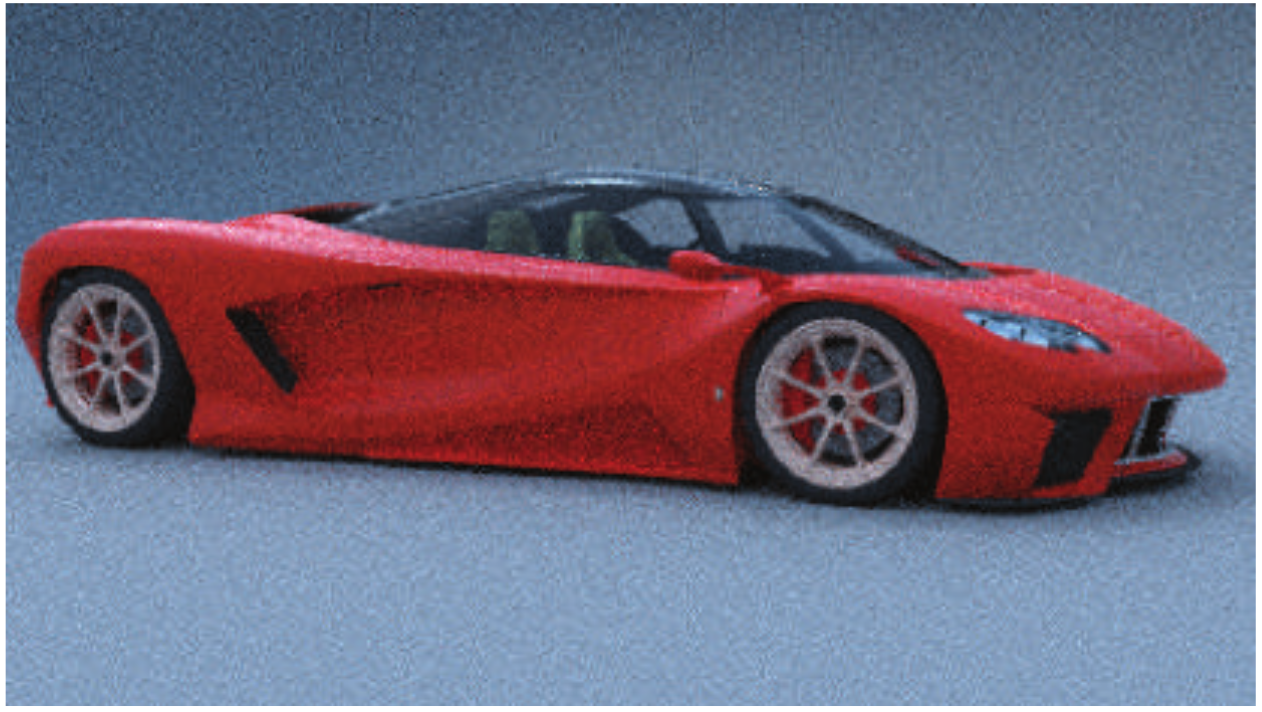
\includegraphics[width=0.7\linewidth]{../assets/chapter6_MC_variance.png}
	\caption{Illustrazione della varianza in una immagine renderizzata. Immagine da \cite{pharr}}
	\label{chapter6:MC:variance}
\end{figure}
Una misura di accuratezza di tale stimatore \`e la sua varianza, la quale si traduce, nell'immagine renderizzata, in variazioni brusche tra pixel 
adiacenti, come mostrato in Figura \ref{chapter6:MC:variance}. Tale varianza\footnotemark{}, per lo stimatore in 
Equazione \ref{chapter6:MC:crudeEstimator}
\begin{align}\label{chapter6:MC:crudeVariance}
	V[\tilde{F}_n]&=V\left[\norm{\mathcal{D}}\tilde{E}_n[f(X)]\right]=\norm{\mathcal{D}}^2V\left[\tilde{E}_n[f(X)]\right]%
	=\frac{\norm{\mathcal{D}}^2}{n}V[f(X)] \\
	&=\frac{\norm{\mathcal{D}}^2}{n}\frac{1}{\norm{\mathcal{D}}}\int_{\mathcal{D}}(f(x)-\bar{f})^2\mathrm{d}x=
	\frac{\norm{\mathcal{D}}}{n}\int_{\mathcal{D}}f(x)^2\mathrm{d}x-\bar{f}^2 \nonumber
\end{align}
Da cui la deviazione standard, la quale rappresenta l'errore dello stimatore di monte carlo, \`e pari a
\begin{equation}
	\sigma[\tilde{F}_n]=\sqrt{V[\tilde{F}_n]}=\sqrt{\frac{\norm{\mathcal{D}}^2}{n}V[f(X)]}=\frac{\norm{\mathcal{D}}}{n^{\frac{1}{2}}}\sigma[f(X)]
\end{equation}
Essa diminuisce come \mbox{$\mathcal{O}\left(n^{\frac{1}{2}}\right)$}, Il che dimostra che il \textit{rateo di convergenza} dello stimatore \`e 
$1/2$. Esso \`e chiamato "diminishing return" dal fatto che 
per abbattere l'errore atteso di un fattore $1/n$ bisogna campionare un numero di campioni pari a $n^2$ volte. Si noti che tecniche di quadratura 
convergono pi\`u velocemente per integrali 1D, ma appena si passa a integrali multidimensionali il loro costo e convergenza peggiorano 
considerevolmente, mentre la accuratezza di Monte Carlo non dipende dalla dimensionalit\`a, rendendolo l'unica alternativa.
\footnotetext{Ricordiamo che $V[aX+b]=a^2V[X]$ e che, se le variabili $\left\{X_i\right\}_{i=1}^n$ sono incorrelate, 
	\mbox{$V\left[\tilde{E}_n[f(X)]\right]=V[X]/n$}}
Altre caratteristiche dello stimatore sono \textit{efficienza}, \textit{bias}, \textit{mse}
\begin{altDescription}{chapter6:MC:estimatorQualities}
	\item[Bias] Aspettazione della differenza tra il valore stimato e lo stimando
		\begin{equation}
			\beta = E[\tilde{F}_n(X)]-\int_{\mathcal{D}}f(x)\mathrm{d}x
		\end{equation}
		Nonostante sembrino sconvenienti, in quanto non tendono al valore desiderato, possono comunque risultare vantaggiosi nel caso si desideri uno
		stimatore con varianza minore. Per esempio, lo stimatore biased per la aspettazione
		\begin{equation}
			\frac{1}{2}\max\{X_1,X_2,\ldots,X_n\}
		\end{equation}
		ha deviazione standard che segue \mbox{$\mathcal{O}\left(n^{-1}\right)$}
	\item[Efficienza] Parametro che permette di stimare la bont\`a di uno stimatore in relazione alla varianza ottenuta $V[X]$ e al suo running time
		$T[X]$, pari a 
		\begin{equation}
			\epsilon[\tilde{F}_n]=\frac{1}{V[\tilde{F}_n]T[\tilde{F}_n]}
		\end{equation}
	\item[MSE]
\end{altDescription}
